\section{Evaluation of \os}
\label{s:eval}



\begin{figure}[tb]
 \setlength{\belowcaptionskip}{-10pt}
 \setlength{\abovecaptionskip}{0pt}
\begin{minipage}[t]{0.48\linewidth}
  \centering 
  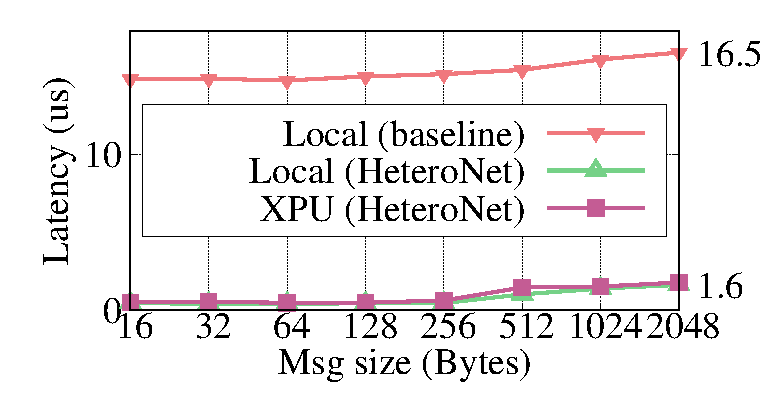
\includegraphics[width=0.99\textwidth]{figs-eval/eval-micro-socket-lat.eps}
  \footnotesize %\\[-5pt]
  \textbf{(a) Latency (small msg).}
  \end{minipage}
\begin{minipage}[t]{0.48\linewidth}
  \centering 
  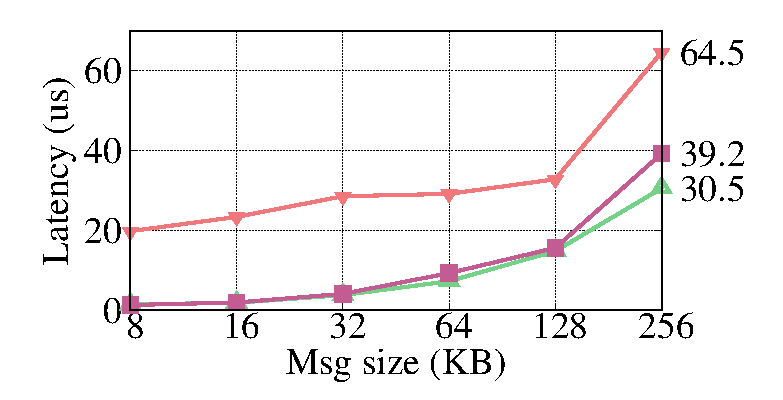
\includegraphics[width=0.99\textwidth]{figs-eval/eval-micro-socket-lat-large.eps}
  \footnotesize %\\[-5pt]
  \textbf{(b) Latency (large msg).}
  \end{minipage}

  \begin{minipage}[t]{0.48\linewidth}
  \centering 
  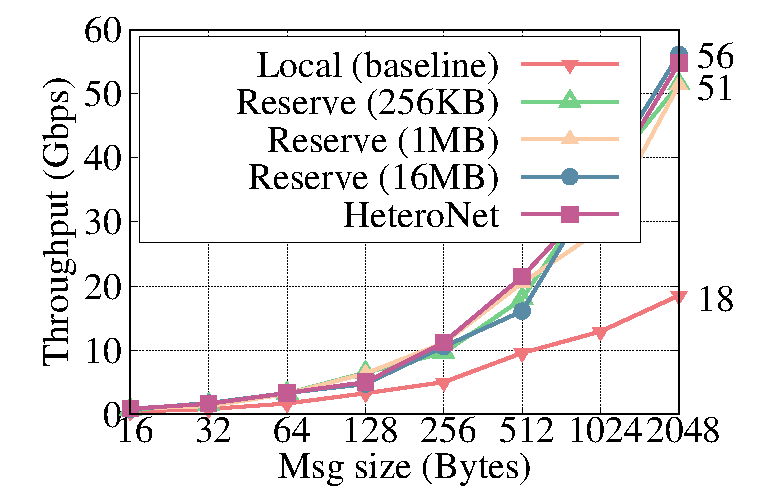
\includegraphics[width=0.99\textwidth]{figs-eval/eval-micro-socket-thr.eps}
  \footnotesize %\\[-5pt]
  \textbf{(c) Throughput (Shm, small).}
  \end{minipage}
\begin{minipage}[t]{0.48\linewidth}
  \centering 
  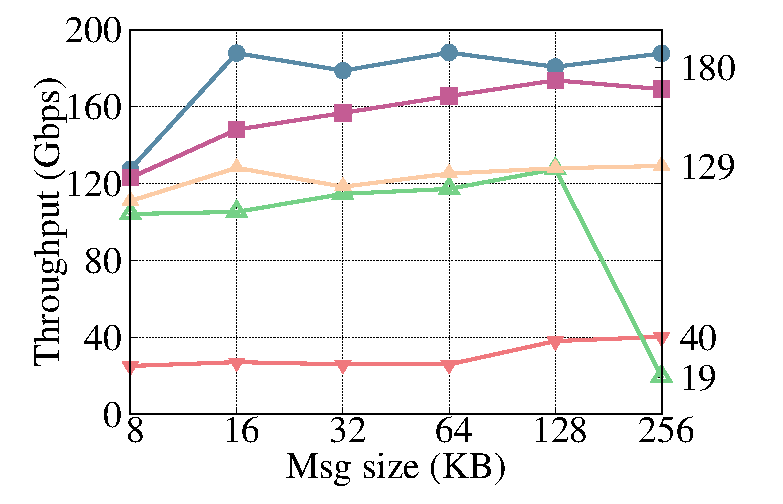
\includegraphics[width=0.99\textwidth]{figs-eval/eval-micro-socket-thr-large.eps}
  \footnotesize %\\[-5pt]
  \textbf{(d) Throughput (Shm, large).}
  \end{minipage}

  \begin{minipage}[t]{0.48\linewidth}
  \centering 
  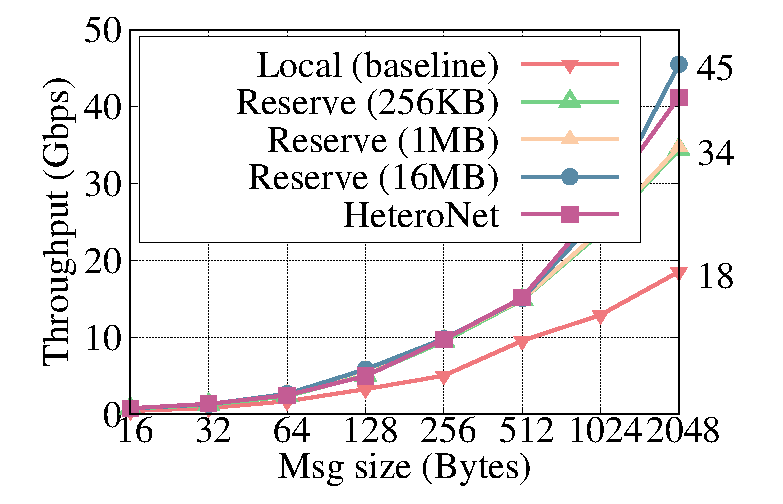
\includegraphics[width=0.99\textwidth]{figs-eval/eval-micro-socket-thr-cxl.eps}
  \footnotesize %\\[-5pt]
  \textbf{(e) Throughput (CXL, small).}
  \end{minipage}
\begin{minipage}[t]{0.48\linewidth}
  \centering 
  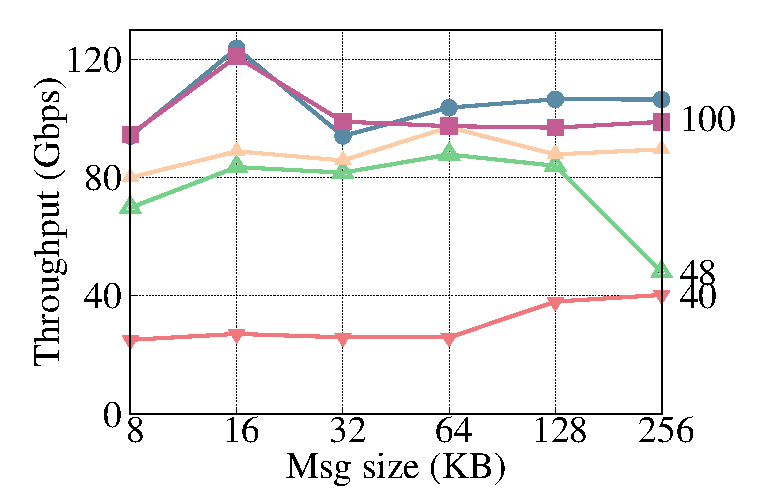
\includegraphics[width=0.99\textwidth]{figs-eval/eval-micro-socket-thr-large-cxl.eps}
  \footnotesize %\\[-5pt]
  \textbf{(f) Throughput (CXL, large).}
  \end{minipage}
	\caption{\textbf{Network performance.}}
  \label{fig:heterosocket-micro}
\end{figure}


\subsection{\gsocket Performance}
\label{subs:eval-socket-microbench}

We conduct an evaluation of network performance with \gsocket. %using CXL-DPU-Sim to compare the network approaches with \gsocket. 
We utilize two test cases, lat\_tcp and bw\_tcp from LMBench~\cite{mcvoy1996lmbench}, to evaluate network latency and throughput. 
We compare three systems:
(1) Baseline is the network performance in a single PU using Linux network,
(2) Reserve is a version of \os that reserves a specific GShm for connection, e.g., 1MB means the connection will reserve two 1MB buffers for use (two directions),
and (3) \os (128KB for local records and 128MB for shared arena).

\myparagraph{Latency.}
Fig.\ref{fig:heterosocket-micro}-a/b shows the results of latency for baseline and \os (local using shared memory and XPU using CXL).
Compared with baseline, \os can achieve 10.1x (2KB) -- 31.9x (16B) better latency for small msgs (in the same PU), and 2.1x (256KB) -- 13.2x (8KB) for large msgs.
For cross-PU cases, CXL-based \os can achieve comparable latency as Shm, and two orders of magnitude better over Cross-PU network baseline (not shown for space reason).
UNAPI takes about 0.51us for cross-PU notification with CXL, and needs additional costs to handle faults and upcall.

\myparagraph{Throughput.}
Fig.\ref{fig:heterosocket-micro}-c/d shows the results of throughput for local-PU (\os using Shm)
and e/f for cross-PU (\os using CXL, still use local-PU results for baseline because cross-PU network is significantly slower).
We also present the results of \os that utilizes fixed reserved buffer (instead of local-records/shared arena design). % including 256KB/1MB/16MB per-connection.
Compared with baseline, \os improves throughput by 1.9x--2.9x for small msgs and 4.8x--6.3x for large msgs on single-PU.
Cross-PU \os (CXL) outperforms single-PU baseline by 1.4x--4.4x.

\myparagraph{Resource costs.}
Assume 1,000 connections in Fig.\ref{fig:heterosocket-micro}-c/d/e/f.
Reserving 16MB will require 16GB pinned resource for communication, which is a non-trivial burden.
Instead, 1MB (1GB total) and 256KB (256MB total, shared by 1,000 connections) can achieve good throughput for small msgs, but show significant slowdown for larger msg sizes ($>$2x worse for 256KB).
\os uses 128KB private records and 128MB shared arena (256MB total), but achieves almost the same good performance as reserving 16MB --- 64x memory saving in this case.
Our practice in real cloud is to reserve 1MB for RDMA (per-connection) and 1MB for traditional Linux TCP,
therefore, the improvement is admirable.





\newcommand{\cmark}{\color[HTML]{32CB00}{\ding{51}}}
\newcommand{\xmark}{\color[HTML]{FE0000}{\ding{55}}}

\begin{table}[]
\setlength{\abovecaptionskip}{0pt}
\centering
%\scriptsize
\footnotesize
% Please add the following required packages to your document preamble:
% \usepackage{booktabs}
\caption{\textbf{LoC of supported applications.}
%\textit{We two of the most intricate applications supported by \os and Molecule~\cite{10.1145/3503222.3507732}. In total, four applications were selected for evaluation. \os can support real-world applications with significant higher Line-of-Code (LoC). {\cmark} denotes supported by Molecule or \os, while {\xmark} signifies unsupported}}
\textit{\os can support real-world applications with significant higher Line-of-Code (LoC). {\cmark} denotes supported by Molecule or \os, while {\xmark} signifies unsupported. CNN image is from FunctionBench, while Alexa is from ServerlessBench.}}
\begin{tabular}{@{}lcccc@{}}
\toprule
\textbf{Applications}    & \textbf{Version}                                                     & \textbf{LoC} & \textbf{Molecule} & \textbf{\os} \\ \midrule
Python3  & 3.8.10                                                               & 1,085,262    & \xmark                 & \cmark                   \\
Envoy                    & \#330dbdc8f9                                                         & 764,457      & \xmark                 & \cmark                   \\ \midrule
CNN image                & \#296f5f2  & 135          & \cmark                 & \cmark                   \\
Alexa smarthome          & \#207b345 & 1,804        & \cmark                 & \cmark                   \\ \bottomrule
\end{tabular} \\[-10pt]
\label{t:eval-efforts}
\end{table}








\subsection{Compatibility}
We analyze the Line-of-Code (LoC) for two of the most intricate applications supported by \sys and Molecule~\cite{10.1145/3503222.3507732},
as shown in Table~\ref{t:eval-efforts}. 
Although frameworks like Molecule utilizes new abstractions to sucessfully support serverless, it is very difficult to support commodity cloud-native apps like Python-based services and Envoy~\cite{envoy} (widely used in service mesh systems).
\sys (with \os) can support commodity apps with significantly higher LoC on CPU-DPU computers,
which is a new milestone.


\myparagraph{Supporting other heterogeneous devices.}
\os is general to other general-purpose heterogeneous devices.
However, for domain-specific accelerators like FPGA and GPU, applications usually do not depend on APIs like socket.
In these cases, we can directly use low-level abstraction, e.g., DMA, for efficient communication.
It is also possible to extend \os with related systems like GPUnet~\cite{kim2014gpunet}, Lynx~\cite{tork2020lynx}, and Coyote~\cite{korolija2020abstractions} in the future.


\myparagraph{Supporting other systems.}
We implement our prototype based on Kubernetes because it is the most widely-used cloud-native platform today~\cite{cncf-landscape}.
Nevertheless, the idea of dynamic split and the techniques (i.e., \giptable and \gsocket) are general.
The implementation can also be applied to other cases besides cloud-native apps.


\myparagraph{Limitations.}
Our prototype supports \gsocket for apps that dynamically linked with libc.
Statically pre-compiled apps are not supported (we can support static compiled apps with re-compilation).
\os mainly focuses on apps cooperate with network.
Prior work~\cite{10.1145/3503222.3507732} has supported the case of IPC, which will be integrated.
Offloading more fine-grained granularity, e.g., threads, is still an open challenge for future work.
More policies and benefits of XPU, e.g., energy-efficiency~\cite{234944}, are valuable to explore, but orthogonal to this work which enables the dynamic split \emph{mechanism}.

